\documentclass[twoside, 11pt, openright]{report}

\usepackage[utf8]{inputenc}
\usepackage{hyperref}

\usepackage{graphicx}
\usepackage{epstopdf}
\usepackage{listings}
\usepackage{calc}

\lstdefinelanguage{CPNML}
{
	morekeywords={colset,var,val,fun,let,in,end},
	morekeywords={union,bool,string,int,unit,enum,index},
	morekeywords={list,record,product,subset,alias},
	sensitive=true,
	morecomment=[s]{(*}{*)},
	morestring=[b]",
	basicstyle=\ttfamily,
	breaklines=true,
	frame=lines
}

\newcommand{\clearemptydoublepage}{\newpage{\pagestyle{empty}\cleardoublepage}}


\newcommand{\fig}[4][0.5]{
	\begin{figure}
	\centering
	\includegraphics[scale=#1]{figures/#2}
	\caption{#3}
	\label{fig:#4}
	\end{figure}
}
\newcommand{\figrot}[4][0.5]{
	\begin{figure}
	\centering
	\includegraphics[scale=#1,angle=90]{figures/#2}
	\caption{#3}
	\label{fig:#4}
	\end{figure}
}
\newcommand{\figref}[1]{Fig.~\ref{fig:#1}}
\newcommand{\lstref}[1]{Listing~\ref{lst:#1}}

\begin{document}
\lstset{language=CPNML,tabsize=1}

\pagestyle{empty}
\pagenumbering{roman}

\vspace*{\fill}
\begin{flushright}
  {\Huge\sf Design and Evaluation of a}\\[2ex]
  {\Huge\sf Framework for Annotating}\\[2ex]
  {\Huge\sf Coloured Petri Net Models}\\[2ex]
  {\Huge\sf with Code Generation Pragmatics}\\[4ex]
  {\huge\sf Mikal Hitsøy Henriksen} 
\end{flushright}
\noindent\rule{\linewidth}{1mm}\\[-.5ex]
\noindent\rule{\linewidth}{2.5mm}
\vfill
\begin{center}
  {\huge\sf Master's Thesis}\\[\fill]
%  
\includegraphics{au-segl.ps}\\[\fill]
  {\sf Department of Computer Engineering\\Bergen University College\\Norway}
\end{center}
\begin{center}
  {\sf \makeatletter\@date\makeatother\\Supervisor\\Lars Michael Kristensen}
\end{center}
\vspace*{\fill}
\clearemptydoublepage



%\chapter*{Abstract}
%\addcontentsline{toc}{chapter}{Abstract}

\begin{abstract}
Model Driven Development

CPN

Under development: Annotations for code generation

Designing and evaluating framework
\end{abstract}


\clearpage
\tableofcontents
\clearemptydoublepage



\pagestyle{headings}
\pagenumbering{arabic}
\setcounter{page}{1}

\chapter{Introduction}
\label{chap:introduction}


\section{Coloured Petri Nets}

\chapter{Background}
\label{chap:background}



\section{Coloured Petri Nets}
Common usage: Process and protocol modeling, concurrent programming. Operations:
Simulation, verification and analysis. More recently also software design.

Short intro to places, transitions and arcs?

\section{CPN Tools}

Graphical tool used to design CPN models. 

Reference, with url

\subsection{Standard ML}

Functional language. (Ref) We will call it SML.
Give examples

\subsection{Declarations}

\section{WebSocket}

This section is about the WebSocket
protocol \cite{draft-ietf-hybi-thewebsocketprotocol}.

\begin{figure}
\centering
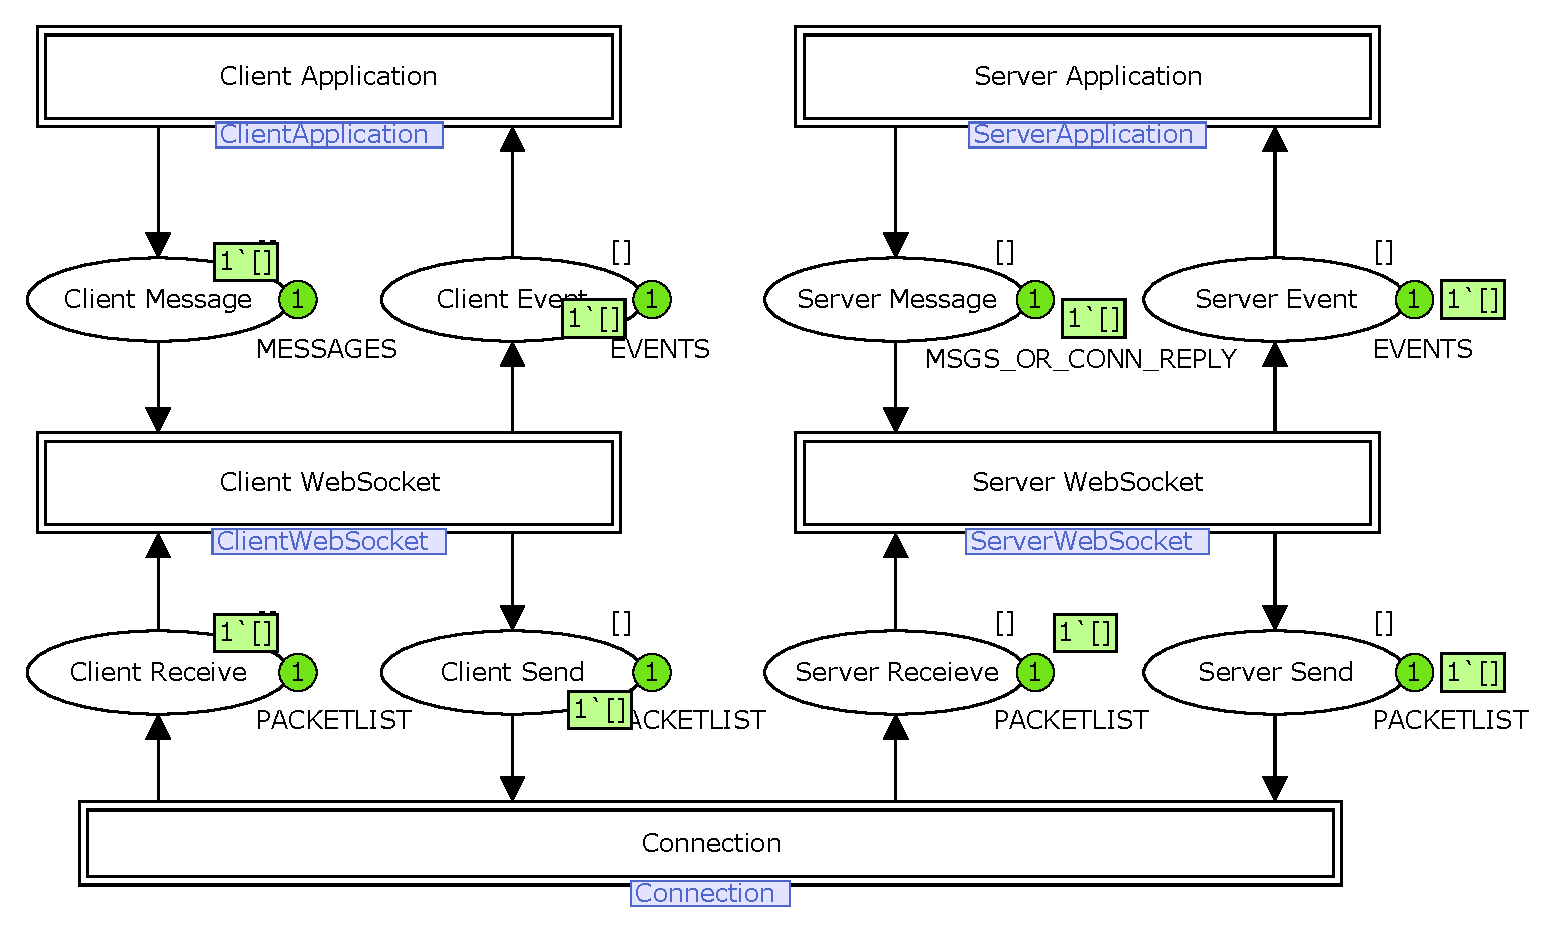
\includegraphics[scale=0.4]{figures/Overview.eps}
\caption{Overview of CPN model of the WebSocket protocol}
\label{fig:overview}
\end{figure}

Shown in Fig.~\ref{fig:overview} is the top-level overview of the WebSocket
protocol as a CPN model. 

Resembles part of OSI model (ref), where top level is levels 6 and 7, middle
level is level 5, and bottom level is levels 4 through 1. Two-way communication
between levels.

Circles represent places. They can contain tokens of a specified colour, and
can have markings to define initial tokens.

Double-bordered represent subpages. These are separate models that have
input and output places that connect to the places on their parent page. We will
examine the first subpage next.

\subsection{Client Application}

\begin{figure}
\centering
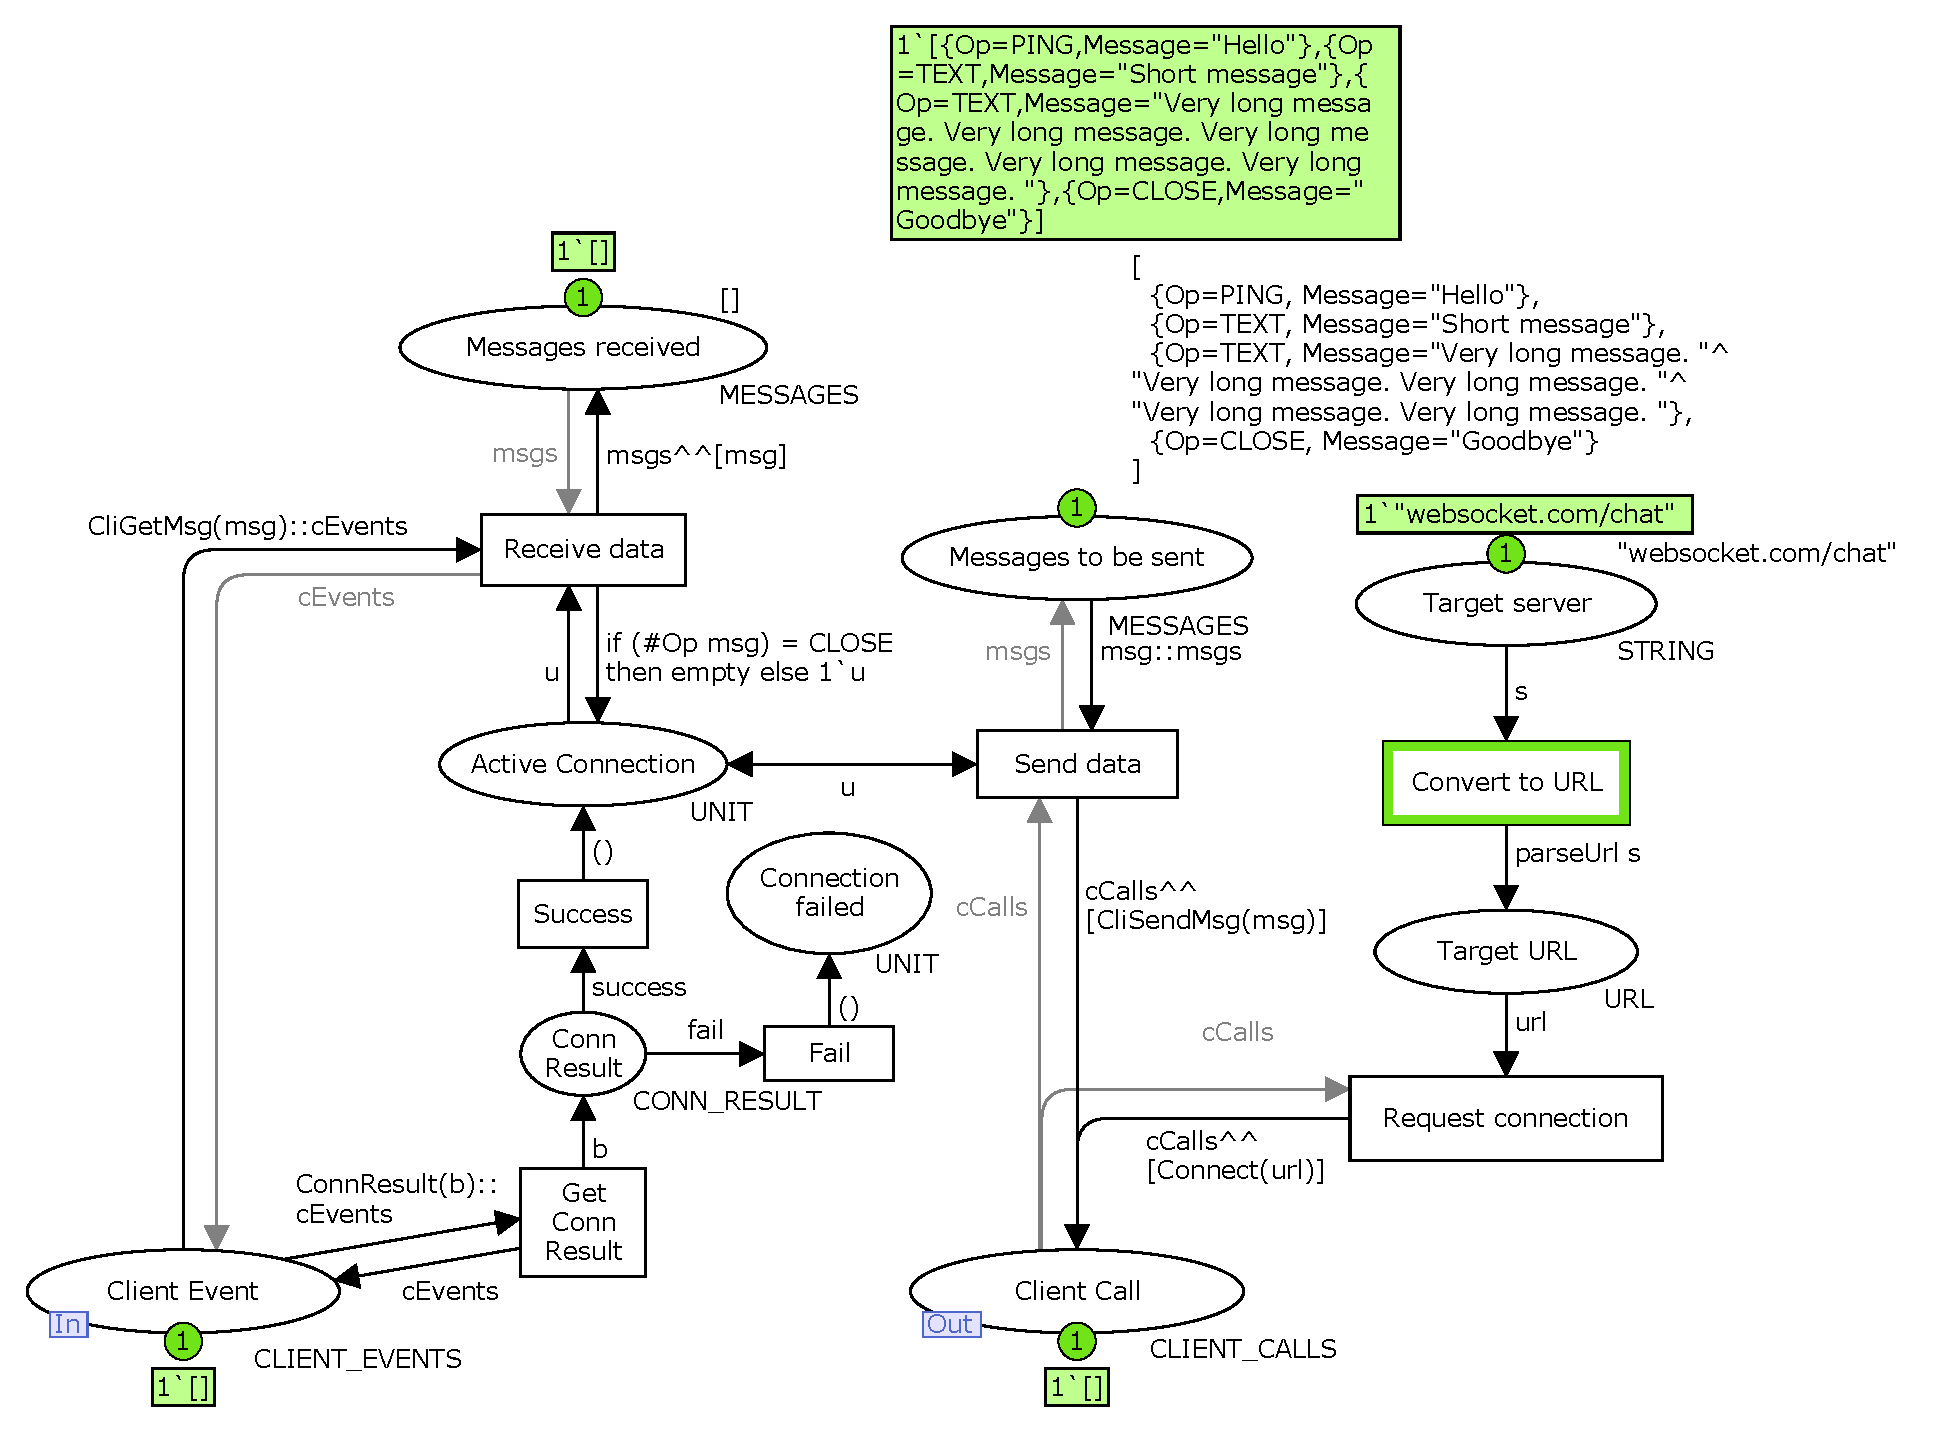
\includegraphics[scale=0.4]{figures/ClientApplication.eps}
\caption{The Client Application}
\label{fig:client_app}
\end{figure}

Laid out from top to bottom to loosely show sequence. 

Bottom places represent interface to WebSocket library. To simplify the overview
model and facilitate easier later expansion, we have only two places that act as
input and output, tagged In and Out. These are connected to the
respective places on the Overview, which are also connected to corresponding places in the
WebSocket Library.

Connect to server
Wait for result
Send and receive data

Here we see an enabled transition at the top. If we were to fire this
transition, it would produce a MESSAGE token in the Send Client Message place.

To the left we see a two-way arc between a place and a transition. This is a
technique used to simulate ordered processing of tokens; queues. We use
lists to do this. To describe a list in SML, we write [] for an empty list and
head::tail for a non-empty list, where head is the first element in the list,
and tail is all the following elements.

So, instead of using the actual color we want in the place, we use a list of
this color. When we want to take an element from the front of the queue,
we use the :: operator to bind the head and tail of the list to variables, and
put only the tail back to the source place. When we want to append an element
to a queue, we concatenate the queue using the \verb|^^| operator with a new
list containing only the new element. To improve readability of the model, these queue operations have
one arc slightly dimmed, to emphasise the flow direction of data.


\subsection{Client WebSocket Library}

\begin{figure}
\centering
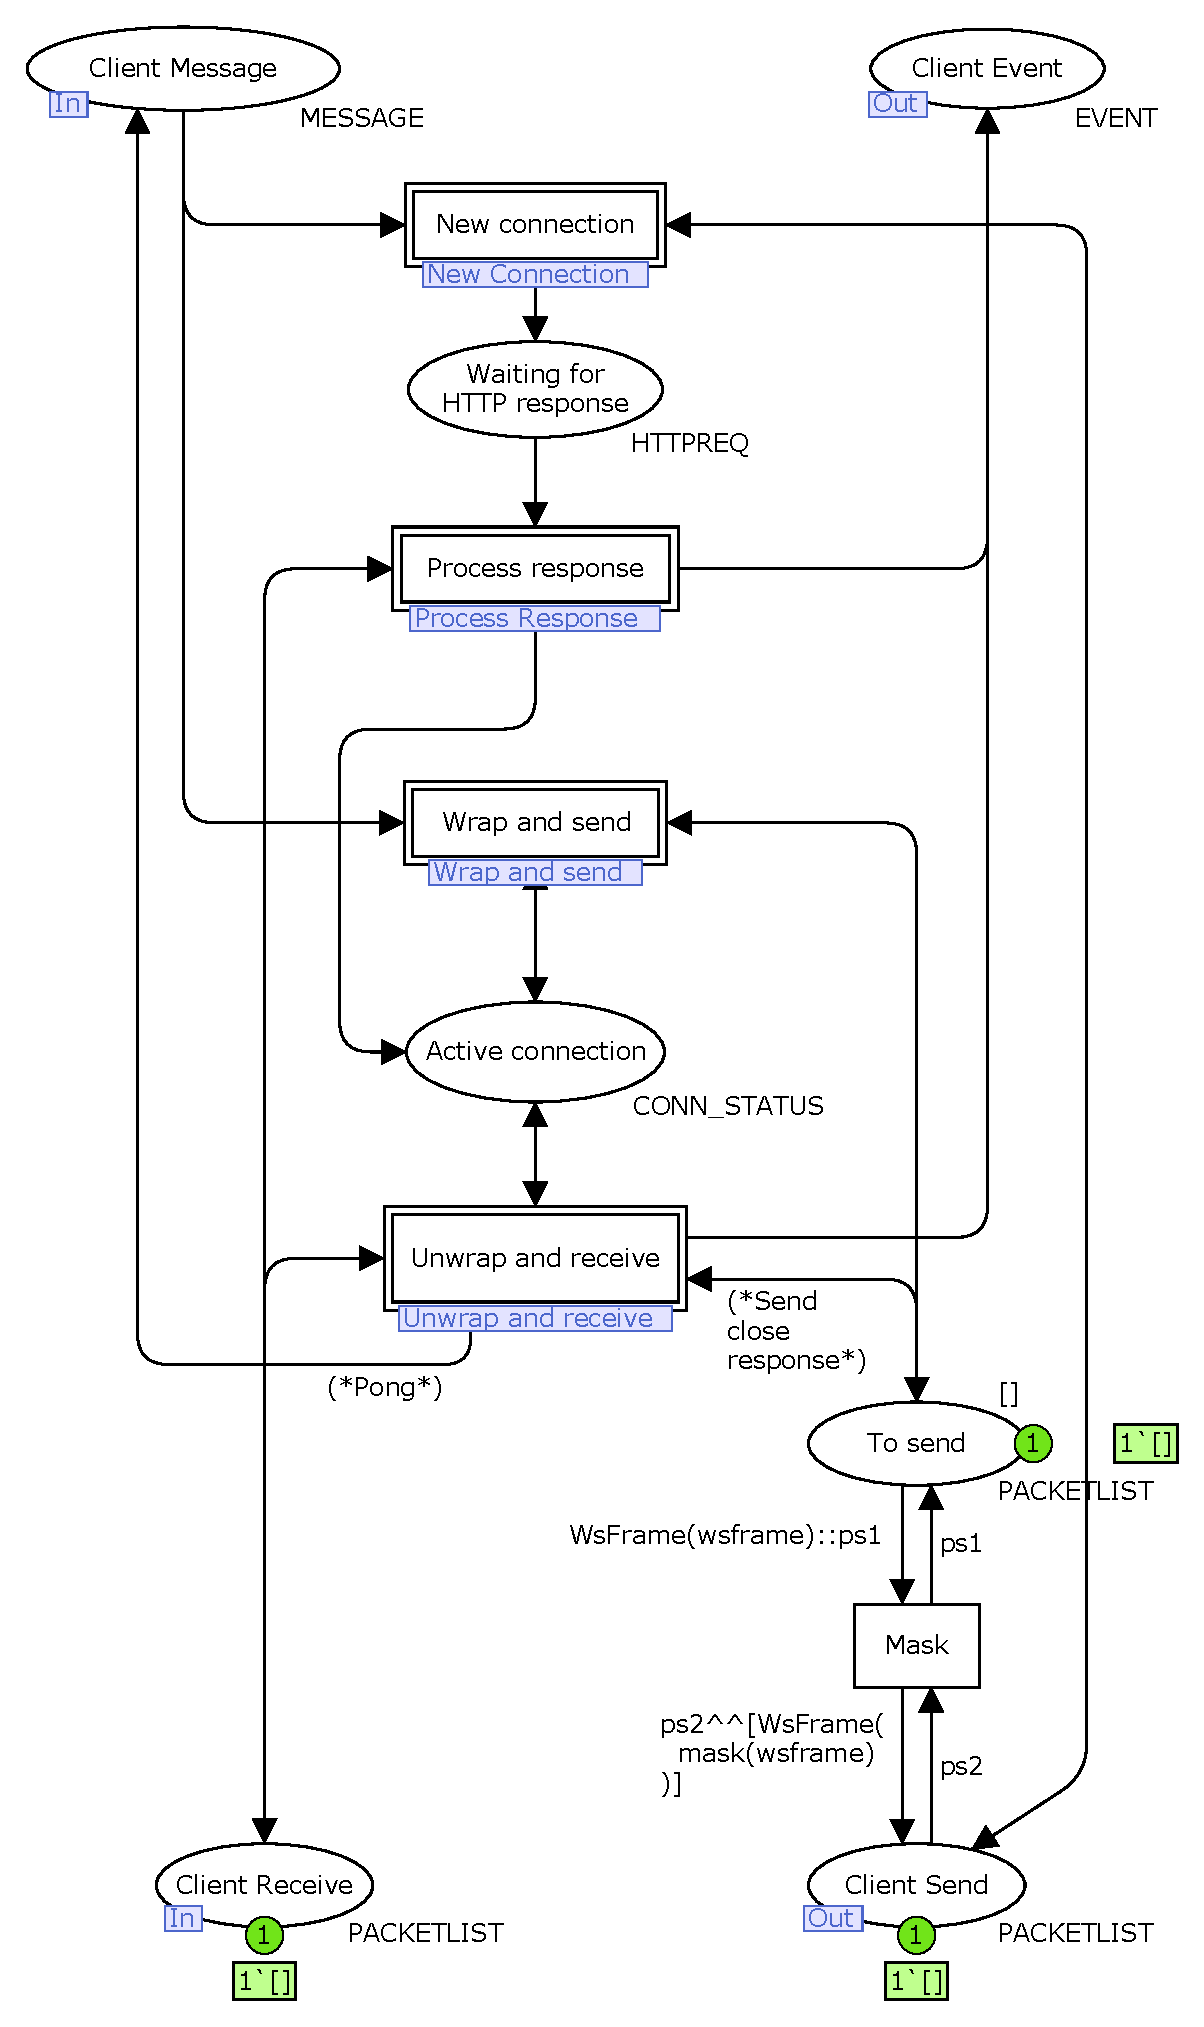
\includegraphics[scale=0.4]{figures/ClientWebSocket.eps}
\caption{The Client WebSocket Library}
\label{fig:client_wslib}
\end{figure}

This page consists mostly of subpages. The only processing being done here is
masking of all websocket frames.

\subsubsection{New connection}



%\chapter{Technology and foundations}
\label{chap:technology}

One of the first decisions that had to be made for this thesis was whether to
base the work on an existing platform or to create a new one from
scratch. In this chapter we will describe the reasoning behind our choices, and
give an overview of the technologies that have been used.

\section{(decision)}\com{Finne på tittel}
	A simple but easy way of manipulating a CPN model is by representing it as a
	tree. Simple tree editors are a feature of most GUI software platforms. Even
	so, we realised early that writing everything from scratch would probably take
	much longer than adapting an existing platform.

	There are of course many complete implementations of Petri Net tools in
	different languages and toolkits, but few of them are open source, or written with
	extensibility in mind. If we were to base our work on an existing platform, it
	would have to be open and extendable. 
	
	To narrow our search, we limited our options to solutions in
	languages we had experience with: Java, c++/Qt and Ruby. Java is a popular
	language, and we already have Access/CPN, a part of the CPN Tools project,
	which can parse .cpn files into Java objects. 
	
	By searching the web, we discovered the ePNK framework, an extendable framework
	for working with Petri Nets in a graphical manner, and lets you specify your
	own Petri Net type. It is built on the Eclipse Modeling Framework (EMF) (which
	Access/CPN is also built on).
	
	We also needed a way to represent pragmatics. It was suggested to try an
	ontology-based approach, and we decided on SADL, another Eclipse plugin that
	lets us easily define and work with ontologies.
	
	\fig{AppOverviewDiagram.pdf}{Application Overview Diagram}{app_overview}
	
	\figref{app_overview} shows the different elements that make up the application.
	The elements with bold frames are the ones newly created for this thesis, while
	the rest below are the existing solutions used and built upon. These will be
	described in the following sections, from the bottom up.

\section{Eclipse IDE}
Eclipse IDE is an open source, cross-platform, polyglot development environment.
Its plugin framework makes it greatly extendable and customisable, and especially makes it
easy for developers to quickly create anything from small custom macros, to
advanced editors, to whole applications. The Eclipse IDE is open source, and
part of the Eclipse Project, a community for incubating and developing open
source projects.

\fig{EclipsePlatformDiagram.pdf}{The Eclipse RCP}{eclipse_rcp}

The Eclipse IDE is built on the Eclipse Rich Client Platform (RCP),
\figref{eclipse_rcp}. At the bottom of this we have the Platform Runtime, based
on the OSGi framework, which provides the plugin architecture. The other
plugins shown in the diagram together form a basic generic IDE.

The principal Eclipse distribution is the Eclipse Java IDE, which is one of the
most popular tools for developing all kinds of Java applications, from small
desktop applications, to mobile apps for Android, to web applications, to
enterprise-scale solutions. 

Plugins are the building blocks of Eclipse, and there exists a wide range of
plugins that add tools, functionality and services. For example, this thesis
was written in \LaTeX{} using the Texlipse plugin, and managed with the Git
version control system through the EGit plugin. 

Publishing a custom plugin is simple. By packaging it and serving it on a
regular web server, anyone can add the web server url to the update manager in
Eclipse, and it will let you download and install it directly, as well as
enabling update notifications.

It is possible to package Eclipse with sets of
plugins to form custom editions of Eclipse that are tailored for specific
environments and programming languages. Aptana Studio is one example, aimed at
Ruby on Rails and PHP development.


\section{Eclipse Modeling Framework}
EMF is a framework for Model Driven Development (MDD) in Java. It is an Eclipse
plugin that is part of the Eclipse Platform, and open source. By providing
modeling and code generation tools, it lets developers create model
specifications that can be converted to Java classes, along with a
set of adapter classes that enable viewing and command-based editing of the
model, and a basic editor. \com{prøve å utvide, men vanskelig å finne noe mer
fornuftig å skrive}

	\subsection{Graphical Modeling Framework}
	GMF builds on EMF to provide graphical viewing and editing of models. It uses
	metamodels created with EMF to generate implementations of views and editors
	that can create and edit the respective models. 

\section{ePNK: Petri Net framework}
ePNK is an Eclipse plugin both for working with standard Petri Net models, and a
platform for creating new tools for specialised Petri Net types, which is
exactly what we need for our annotated CPN. It uses EMF and GMF to work with the
Petri Net models and provide generic editors for custom Petri Net variants.

There are several reasons why ePNK is a good choice:
\begin{itemize}
	\item It saves models using the ISO/IEC 15909 \com{referanse?} standard file
	format PNML,
	\item It is currently actively developed,
	\item It is designed to be generic and easily extendable by creating new model
	types, and
	\item It includes both a tree editor and a graphical editor, provided through
	GMF.
\end{itemize}

ePNK includes definitions for the core PNML model type, as well as two
subtypes of Petri Nets. The first is P/T-Nets, or Place/Transition Nets, which
expand on the core model with a few key items: initial markings for places,
inscriptions on arcs, and constraining arcs to only go between a place and a
transition (this is not enforced in PNML, as there are Petri Net variants that
allow this). 

The other is High level Petri nets (HLPNG). This type adds several more labels,
all of which are Structured Labels. These are parsed and validated using a
syntax that is inspired from (but not the same as) CPNML from CPN Tools. It is
possible to write invalid data in these labels and still save the document, as
they will only be marked as invalid

Neither of these two conform exactly to the Coloured Petri Nets created by CPN
Tools. HLPNG comes close, but is missing a few things like ports and sockets
(RefPlaces can emulate this), and substitutin transitions. Also, the
structured labels are not compatible with CPNML syntax from CPN Tools, and for
our prototype, these structured labels are not necessary with regard to
annotations. It is possible that this might be useful in a future version,
where for example pragmatics are available depending on things like the
colorset of a place or the variables on an arc, but this would take too much
time to implement. \com{Bedre formulering av siste setning?}

Our decision was to develop our own Petri net type, which matches CPN Tools as
close as possible.

\section{Access/CPN: Java interface for CPN Tools}
CPN Tools has a sister project called Access/CPN. This is an
EMF-based tool to parse .cpn files and represent them as an
EMF-model. The .cpn files saved by CPN Tools are XML-based, which makes them
easy to parse, but having an existing solution for this is preferrable.

The model definition used by Access/CPN is very similar to that of ePNK.
\com{Diskutere mer i implementation?}

TODO: Vurdere å utvide med egen algoritme som konverterer direkte til ePNK?

\section{SADL: Ontologies}
Ontologies are a way to present information and meta-information so that it can
be understood by computers. Essentially, this is done by defining classes that
have properties, relations and constraints, and then association
information with these classes.

There is a lot of ongoing research on this subject, especially to create a
semantic web, that is extending web pages to provide meta-information about the
content they contain and enabling software to understand it and reason about it. 

SADL is an Eclipse plugin that defines an english-like syntax for defining
ontologies, and comes with a text editor that features syntax highlighting,
parsing and validation. This is useful as we can possibly reuse the editor in
our plugin for defining model-specific pragmatics.

It also has tools to parse and reason with these ontologies, which we will use
to filter and validate which pragmatics are available for different model
entities.

\section{Summary}
After picking these technologies, since all the componets have Eclipse in
common, it was an easy decision to develop our project as an Eclipse plugin.
This also let us centralise all our development in Eclipse.

%\chapter{Analysis and Design}
\label{chap:analysis}

Lorem ipsum dolor sit amet, consectetur adipiscing elit. Sed elit purus, cursus eget pellentesque et, tristique id neque. Sed non quam ac sem malesuada aliquet vitae in massa. Donec a lectus enim, a porttitor velit. Sed rutrum risus non sem ultricies sit amet sollicitudin elit consequat. Quisque tincidunt vulputate lacus, id ornare nisi porta sit amet. Ut congue leo eget nisl semper lacinia. Etiam vitae tortor at diam rhoncus convallis. Vestibulum id metus ante.

\section{Analysis}

Donec sapien tellus, luctus vel molestie ut, pulvinar et tellus. Nunc cursus hendrerit egestas. Etiam pellentesque condimentum metus ut rhoncus. Maecenas eu leo velit, vitae lobortis augue. Pellentesque ullamcorper est ut felis ultricies eu pharetra neque pharetra. Praesent vitae sapien quis ligula hendrerit sagittis id ut sem. Praesent orci quam, molestie vestibulum eleifend id, laoreet tempus dolor. Duis in enim vitae ante mattis molestie vitae imperdiet justo. Sed lorem erat, mollis consequat molestie sit amet, lacinia vulputate lectus. Nunc risus metus, rutrum sit amet aliquet ut, faucibus quis urna. Vestibulum ac turpis ante. Aliquam mauris magna, volutpat malesuada bibendum sed, tempor a magna. Morbi erat enim, vestibulum at mattis eget, dictum at magna.

Morbi ullamcorper enim eu odio gravida et convallis augue feugiat. Ut ut suscipit lorem. Donec tristique facilisis velit, fermentum lobortis massa vestibulum nec. Mauris scelerisque dignissim scelerisque. Duis eu sem dui. Nulla et tortor non urna accumsan congue. Donec neque justo, vestibulum id dignissim venenatis, cursus eu orci. Phasellus vitae placerat mi. Cum sociis natoque penatibus et magnis dis parturient montes, nascetur ridiculus mus.

\section{Design}
Ut nibh massa, faucibus bibendum tempus adipiscing, pretium ac nunc. Cras id imperdiet urna. Suspendisse potenti. Vestibulum hendrerit laoreet arcu, eu congue velit mattis id. Proin aliquam elementum diam sed placerat. Nam mollis mauris id tortor iaculis scelerisque. Nam vel tortor et nunc condimentum dignissim. Fusce ut leo id eros consectetur pharetra at non velit. Vestibulum hendrerit purus quis libero euismod adipiscing. Integer bibendum fermentum viverra. Pellentesque fermentum sapien et eros dignissim pellentesque elementum felis ornare.

Cras scelerisque bibendum convallis. Maecenas laoreet imperdiet lacinia. Fusce ornare augue vitae tortor scelerisque ut rhoncus enim mollis. Quisque non justo mauris. Quisque dolor nulla, feugiat a fringilla sit amet, tempus in dui. Nulla facilisi. Fusce sodales diam quis risus ultricies posuere. Integer et semper mi. In hendrerit tortor a dolor faucibus posuere.

%\chapter{Implementation}
\label{chap:implementation}

Lorem ipsum dolor sit amet, consectetur adipiscing elit. Sed vulputate ornare sagittis. Nam rutrum condimentum dolor at bibendum. Quisque quis massa tellus. Sed luctus mauris sit amet metus lacinia eleifend. Mauris malesuada tellus eget dui convallis id porttitor diam porta. Sed mollis velit a quam condimentum euismod. Sed hendrerit neque et nulla suscipit ac eleifend arcu congue. Suspendisse nisi mi, accumsan non elementum nec, aliquam sed justo. Vivamus eu arcu lorem. Vestibulum a ante nibh, a dignissim lorem. Etiam laoreet ante a est blandit a pellentesque lorem laoreet. Phasellus id velit mauris, et lacinia purus. Sed sodales iaculis vulputate.


\section{Conversion from CPN Tools to ePNK}
Fusce pellentesque, mauris nec fermentum vehicula, ligula turpis dictum ante, ac gravida erat orci vitae libero. Sed ac tellus eros. Nulla facilisi. Suspendisse potenti. Nullam massa leo, viverra at imperdiet id, interdum a nibh. Integer convallis aliquet dapibus. Phasellus sed nisl erat. Curabitur at lacus ligula, non lobortis velit. Suspendisse potenti. Curabitur in velit in est cursus commodo.

Vestibulum in nisi eu risus euismod dapibus. Nam vel lorem ipsum, vel mollis mi. Morbi sed velit sit amet enim commodo fringilla. Nunc dui ante, sodales eget mollis a, commodo porta elit. Fusce urna est, aliquet a pellentesque sit amet, vehicula nec leo. Morbi in dui leo. Class aptent taciti sociosqu ad litora torquent per conubia nostra, per inceptos himenaeos. Ut purus magna, consequat vel semper eget, hendrerit ut massa. Maecenas pulvinar lacus a neque pulvinar congue. Ut malesuada commodo erat, non posuere massa fermentum ut. Proin suscipit sodales bibendum. Ut id dolor mauris, commodo eleifend neque. Etiam interdum interdum euismod. Ut lobortis malesuada pellentesque. Nullam venenatis volutpat ornare. Donec varius elit at elit adipiscing lobortis.

\subsection{Access/CPN}
Aliquam erat volutpat. Praesent ullamcorper commodo augue in faucibus. Sed et tortor non arcu aliquam pharetra. Sed odio massa, pharetra ut faucibus sed, rhoncus vel lectus. Morbi consequat purus at ipsum placerat vel dapibus justo dignissim. Etiam feugiat pulvinar tempus. Fusce vestibulum odio a leo porttitor at pulvinar velit egestas. Praesent at venenatis lectus. Donec gravida, lacus vitae tincidunt tincidunt, risus leo congue mi, vitae pharetra magna ipsum eget dui. Suspendisse suscipit mollis pellentesque. Nunc ac nulla sit amet diam tincidunt volutpat quis in eros. Integer diam odio, mollis ac porta eget, faucibus vel mi. Maecenas vitae mauris tellus. Aliquam vel fringilla arcu. Praesent ut magna massa, ut dignissim massa.

Aenean porttitor massa non quam euismod laoreet. Nam quis nulla sem. Donec hendrerit, orci a ultrices viverra, orci mi ultricies nibh, eu vestibulum nulla eros ac ligula. Donec velit nisi, rhoncus nec pharetra sit amet, pretium sit amet turpis. Nullam scelerisque elit eu nisi vulputate vel imperdiet odio luctus. Maecenas laoreet ante ac elit consequat ullamcorper. Nunc lorem tellus, hendrerit luctus pulvinar tempus, molestie nec mi. Nam sem sapien, aliquam imperdiet tincidunt eu, elementum eu ipsum. Curabitur sed risus at lacus tincidunt rutrum. Praesent id lorem mi. Pellentesque habitant morbi tristique senectus et netus et malesuada fames ac turpis egestas.

%\chapter{Evaluation}
\label{chap:evaluation}

Lorem ipsum dolor sit amet, consectetur adipiscing elit. Maecenas faucibus libero at lorem accumsan at ullamcorper tellus facilisis. Nulla nec metus ligula. Vivamus varius est vitae nisl bibendum porttitor. Suspendisse arcu orci, rhoncus et accumsan non, hendrerit id urna. Aliquam dictum molestie quam, ac imperdiet dui hendrerit in. In posuere laoreet faucibus. Cras sit amet dui risus, gravida condimentum diam. Nullam turpis lacus, lobortis a egestas ac, ultrices et nisl.


\section{Requirements}
Curabitur consequat odio vel dui laoreet rutrum. Praesent pretium lorem a nibh tempus non elementum sem varius. Sed bibendum quam elementum diam vehicula at tempus ipsum cursus. Mauris dui tellus, luctus non tincidunt ac, placerat sit amet metus. Class aptent taciti sociosqu ad litora torquent per conubia nostra, per inceptos himenaeos. Aliquam nec sem ac purus condimentum facilisis. Pellentesque eu libero nec mi faucibus bibendum. Aliquam erat volutpat. Proin id dignissim nunc. Vivamus porttitor pharetra ipsum, in luctus tellus fermentum luctus. Mauris tristique, justo vel blandit venenatis, elit ante volutpat ligula, vitae lobortis nisl magna nec risus. Nullam ultricies porttitor leo non mattis. Pellentesque habitant morbi tristique senectus et netus et malesuada fames ac turpis egestas.

Phasellus imperdiet, dolor feugiat iaculis pharetra, orci nisi blandit mi, sed consectetur justo tellus suscipit eros. Donec non leo purus. Nulla feugiat lorem ut nunc blandit in rhoncus justo lobortis. Nulla facilisi. Vivamus urna mauris, volutpat vitae facilisis nec, aliquet vitae mi. Nullam in ante sem, nec malesuada est. Etiam pharetra eleifend sagittis. Vestibulum id enim nec eros rhoncus consequat id ut diam. Nulla cursus ultricies velit eu vehicula. Aenean luctus augue eget mauris tempor accumsan. Maecenas purus enim, mollis quis aliquam quis, placerat ac purus. Vestibulum quis lectus velit, sed ultrices ligula. Maecenas eget porttitor tortor. Pellentesque ut lorem ipsum.

\section{User Feedback}
Vivamus vitae mi quam, vitae fermentum elit. In blandit nulla quis metus vulputate ultricies. Integer malesuada sagittis interdum. Maecenas vestibulum tortor risus, id ultrices massa. Aenean pharetra velit vel enim euismod a sodales odio euismod. Curabitur nisi mi, feugiat vitae sollicitudin non, porta eget nisi. Nulla mollis, dui id bibendum molestie, augue ante gravida dolor, a laoreet sem est sollicitudin elit. Quisque ac purus leo.

Aenean eget urna eu sapien tincidunt lobortis. Duis id dolor quam, vel feugiat libero. Duis tempor, sem id feugiat consectetur, ante nibh convallis quam, hendrerit hendrerit dolor dui in velit. Proin sagittis ante in nisi tempor vel commodo augue bibendum. Proin eu quam id lectus tristique luctus. Donec a risus ut erat tristique posuere ut eu magna. Phasellus suscipit mi vel ipsum pretium elementum in blandit nisi.

%\chapter{Conclusion}
\label{chap:conclusion}

With \thename{}, we have constructed a fully functional proof of concept that
demonstrates the advantages and disadvantages of using ontologies to manage code
generation pragmatics and applying them to a CPN model. As shown in Chapter
\ref{chap:analysis}, this prototype meets all of the requirements in Section
\ref{sec:requirements}. Through our evaluation by using it to annotate CPN
models of different sizes, we have shown that using ontologies gives a highly
expressive means to defining pragmatics as well as providing automatic
validation of the annotated model. However ontology reasoning using CWA yields
decreasing performance as model size increases, to a point that makes our
prototype unusable for the WebSocket CPN model. Still, we believe our approach
has potential, and warrants further optimisation and research.

\section{Future work}

Continue the work of Simonsen, defining more general and domain-specific
pragmatics. Also, assert required configuration arguments.

Finding or developing ontology reasoner tailored for CWA.

A specialised tool for creating model specific pragmatics would have been ideal.
Such a tool would give simple mechanics using GUI controls for specifying which
model elements a pragmatic can be attached to, and which parameters it has. The
Plugin Manifest editor is a good example of what we have in mind. However, this
could not be included for this thesis due to time constraints.

Implement structured labels for the CPN Type. Could enable placement of
pragmatics inside expressions.

When importing, let user choose between CPN and Pragma CPN. Alternatively,
mechanic for upgrading the Type.

Accurately model sub-modules, ports and sockets. This enables more advanced
pragmatics; for instance the Principal pragmatic could be specified to only be
available for substitution transitions on top-level modules.

\section{Acknowledgments}

Thank supervisor Lars Michael Kristensen

Kent Inge Fagerland Simonsen 

Michael Westergaard for help with Access/CPN

Ekkart Kindler for extensive help with ePNK

%\appendix
\bibliographystyle{alpha}\bibliography{literature,rfc}
%\listoffigures
%\lstlistoflistings


\end{document}
